\problem[Haberman 5.4.2a (5pts)]

Davisson and Germer obtained a (first order, $n=1$) peak of diffracted
electrons at (approximately) 50\Deg (measured from the surface normal)
for an acceleration potential of 54\,V.

\solution{

From the Bragg formulas $n\lambda = 2d \sin \theta = D \sin \phi$, with $n=1$,
the fact that $2\theta = 180\Deg - \phi$, and equation \eqref{eq1} we have

\begin{align*}
  d   &= \frac{D \sin \phi}{2\sin \theta} \qquad \bigg| \qquad \phi
       = 50\Deg \mc \theta = 65\Deg \mc D=0.215\u{nm}\\
      &= \frac{0.76604}{2(0.906308)} (0.215\u{nm})\\
      &= (0.4226)(0.215\u{nm})\\
      &= \boxed{0.091\u{nm} .}
\end{align*}

Note that Figure~\ref{fig1} is rather dull, but at least this hyperlink is a subtle shade of blue. Alternatively, making use of the acceleration potential, the de Broglie relation $\lambda = \Frac{h}{p}$, and the fact that momentum
$p = \sqrt{2 m_e e V}$, we have
%
\begin{align}
  \lambda  &=\frac{h}{\sqrt{2 m_e e V}} \\
      &=\frac{6.626068 \e{-34} \label{eq1} \u{m$^2$kg/s}}{\sqrt{2(9.109\e{-31}\u{kg})(1.602\e{-19}\u{C})(54\u{V})}}\\
      &=\frac{6.626068 \e{-34} \u{m$^2$kg/s}}{\sqrt{1.576002744\e{-47} \u{m$^2$kg$^2$/s$^2$}}}\\
      &= 1.668954\e{-10}\u{m}
\end{align}

\begin{mathtable}[caption=true,title={A table.},label={two}]{ccc}
  \a & \b & \c\\
  \midrule
  \d & \ep & \t\\
\end{mathtable}

We also note that verbatim code must be inserted via the
\texttt{\textbackslash input} command:%

\begin{verbatim}
	\begin{figure}[ht!]
		\vspace{0pt}
		\centering
		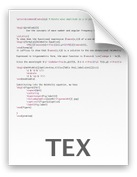
\includegraphics[width=1in]{figure.jpg}
		\caption{A figure.}
		\label{figure2}
	\end{figure}
\end{verbatim}
}